\documentclass[conference]{IEEEtran}
\IEEEoverridecommandlockouts
% The preceding line is only needed to identify funding in the first footnote. If that is unneeded, please comment it out.
\usepackage{cite}
\usepackage{amsmath,amssymb,amsfonts}
\usepackage{algorithmic}
\usepackage{graphicx,booktabs}
\usepackage{textcomp,url,hyperref}
\hypersetup{
    colorlinks=true,
    citecolor=blue,
    filecolor=blue,
    urlcolor=blue,
    pdfpagemode=FullScreen,
}
\usepackage{xcolor}
\def\BibTeX{{\rm B\kern-.05em{\sc i\kern-.025em b}\kern-.08em
    T\kern-.1667em\lower.7ex\hbox{E}\kern-.125emX}}

\begin{document}
    \makeatletter
    \newcommand{\linebreakand}{%
      \end{@IEEEauthorhalign}
      \hfill\mbox{}\par
      \mbox{}\hfill\begin{@IEEEauthorhalign}
    }
    \makeatother

\title{Forex Forecasting*\\
{\footnotesize \textsuperscript{*}Note: All authors contributed equally to this project}
}

\author{\IEEEauthorblockN{Eustathios Kotsis}
\IEEEauthorblockA{\textit{StudentID: 7115152200008} \\
\textit{efstathkot@di.uoa.gr}\\
}
\and
\IEEEauthorblockN{Michael Darmanis}
\IEEEauthorblockA{\textit{StudentID: 7115152200004} \\
\textit{mdarm@di.uoa.gr}\\
}
\and
\IEEEauthorblockN{Vasilios Venieris}
\IEEEauthorblockA{\textit{StudentID: 7115152200017} \\
\textit{vvenieris@di.uoa.gr}
}
}
\newcommand{\ra}[1]{\renewcommand{\arraystretch}{#1}}
\maketitle

\begin{abstract}
The foreign exchange (forex) market, a complex and volatile entity, has been a subject of extensive research, especially in the domain of predicting currency movements. With only 2\% of retail traders successfully predicting currency movement, the challenge is evident. This study implements two variants of machine learning and its statistical models in forex market forecasting. Through a hybrid implementation of RNNs, CNNs, and Exponential Smoothing, we observed that the purely statistical methods often outperformed the hybrid models, especially when sufficient, and good quality data was not available.
\end{abstract}

\begin{IEEEkeywords}
time series analysis, forex forecasting, exponential smoothing, vector autoregression, convolutional neural netwrorks, recurrent neural networks, hybrid methods 
\end{IEEEkeywords}

\section{Introduction}

The forex market stands as the world's largest financial market, with a daily volume surpassing \$6.6 trillion. Its non-centralised nature, operating 24 hours a day, sets it apart from other financial markets. The inherent high volatility, nonlinearity, and irregularity make the forex market one of the most intricate to navigate\cite{ayitey}. Traders in this market deal with currency pairs, comparing the value of one currency to another. Over the years, two primary techniques, fundamental and technical analysis, have been employed for forecasting. However, with the advent of machine learning, a surge in research activity has been observed, aiming to take advantage of these advanced models for more accurate forex-market predictions.

\section{Previous Work}

The realm of forex-market-forecasting, using machine learning, has witnessed significant contributions. Fletcher\cite{fletcher} emphasised the efficacy of discriminative techniques like Support Vector Machines (SVM), Relevance Vector Machines (RVM), and Neural Networks when integrated with advanced exogenous financial information. Panda et al.\cite{panda} conducted an SLR on Exchange Rate Prediction, introducing novel models like Artificial Neural Network (ANN) and Support Vector Regression (SVR). Their findings highlighted the potential of these models in predicting exchange rate projections.

Islam et al.\cite{islam} explored the recent advancements in FOREX currency prediction using machine-learning algorithms. Their research, spanning from 2017 to 2019, revealing a growing academic interest in neural network models and optimisation methodologies. Deep learning algorithms, especially the gated recurrent unit (GRU) and long short-term memory (LSTM), emerged as promising contenders in time series prediction.

Ryll \& Seidens\cite{ryll} undertook a comprehensive review of over 150 publications on machine learning in financial market forecasting. Their analysis suggested that machine-learning algorithms, particularly recurrent neural networks, outperformed traditional stochastic methods in financial market forecasting.

Based on the above insights, our approach focused on using the strengths of Exponential Smoothing\cite{brown}, a purely statistical model, in conjunction with the capabilities of RNNs and CNNs, in order to develop hybrid models suitable for forex-forecasting. A Vector Autoregression model was also employed to benchmark our data.

\section{Our Approach}

Our initial approach to forex-market-forecasting lied on neural models. The  aim was to supplement them with statistical methods. However, the results from this combination were mediocre at best. We then reconsidered our strategy. Instead of primarily relying on a neural model, we turned to the Holts-Winter exponential smoothing technique\cite{winters}, a well-regarded statistical forecasting method. Using this as a foundation, we then looked into enhancing its predictive power by incorporating Recurrent Neural Networks (RNNs).

The second approach actually made a lot of sense. While the Holts-Winters model has its merits, it inherently assumes that the underlying trend in the data is linear\cite{winters}. Forex markets are, by their very nature, dynamical systems whose trends often exhibit non-linear characteristics\cite{ayitey}. Thus, incorporating an RNN architecture for the level seemed like the way to go.

In the following part of the report, we will briefly summarise how these two hybrid models work, how we assessed their performance, the experiments performed and the conclusions drawn thereof.

\section{Hybrid Models}

\subsection{Smoothed Convolutional Neural Networks (S-CNN)}

As mentioned earlier, the core idea here was to enhance the CNN's ability of forecasting by using a purely statistical method. For that purpose we used a simple exponential smoothing technique, which enhances forecasting accuracy\cite{e-cnn} by calculating an average of previous values. The simplest form of exponential smoothing is given by Equation~\ref{eq:ses}:
\begin{equation}
\displaystyle s_{t}=\alpha x_{t}+(1-\alpha )s_{t-1}=s_{t-1}+\alpha (x_{t}-s_{t-1}) .\label{eq:ses}
\end{equation}
Note that the significance of past observations diminishes exponentially as one moves further into the historical data. Wibawa et al.\cite{e-cnn} method  particularly beneficial for erratic and fluctuating datasets.

Initially, the data undergoes "exponential smoothing," emphasising recent observations, while gradually reducing the weight of older data, effectively reducing noise and capturing the primary trend.

Post-smoothing, individual CNNs are trained for every single time series, allowing the model to thoroughly learn each serie's distinct characteristics. These CNNs are not only designed to predict the next value, but also to forecast multiple future points simultaneously.

\subsection{Exponential Smothing Recurrent Neural Networks (ES-RNN)}

This approach takes from the ES-RNN algorithm, winner of the M4-competition\cite{m4}, discussed in detail in a blog post by Slawek \cite{slawek}. The algorithm is divided into two distinct layers: a pre-processing layer that uses exponential smoothing and a LSTM layer that updates the per-series parameters of the Holts-Winter model.

In the pre-processing layer, Holts-Winter exponential smoothing \cite{winters} with multiplicative seasonality and trend is applied via
\begin{align}
    l_t &= \alpha(\frac{y_t}{s_{t-m}}) + (1 - \alpha)l_{t-1} b_{t-1} \label{eq:level}\\
    b_t &= \beta(\frac{l_t}{l_{t-1}}) + (1- \beta) b_{t-1} \label{eq:trend} \\ 
    s_{t} &= \gamma \frac{y_t}{l_{t-1} b_{t-1}} + (1-\gamma)s_{t-m} \label{eq:season}\\
    \Hat{y}_{t+h} &= l_t  b_t^h s_{t-m+h^+_m} \label{eq:predEq}
\end{align}
where $l$ is a state variable for level, $b$ is a state variable for trend and $s$ is a multiplicative seasonality coefficient. $\alpha, \beta$ and $\gamma$ are smoothing coefficients between zero and one. An $h$ step forecast is given by Equation \ref{eq:predEq}.

Since the model no longer considers local linear trend\footnote{remember, that is one of the caveats of the Holts-Winters model}, Equation \ref{eq:trend} is replaced by an RNN from the model as follows:
\begin{align}
    \Hat{y}_{t+1 \dots t+h} &= RNN(X_t) * l_t * s_{t+1 \dots t+h} \label{eq:modifiedEq}\\
    x_i &= \frac{y_i}{l_t s_i} \label{eq:x}
\end{align}
$X_t$ is a vector of normalised\footnote{normalised using the level}, de-seasonalised features of which a scalar component $x_t$ is calculated via Equation \ref{eq:x}.

It is important to note that the RNN and the classical Holts-Winters parameters detailed are jointly trained. The power of the ES-RNN\cite{es-rnn} lies in the co-training of both the per-time series Holts-Winters parameters and the general RNN parameters.

So, to sum up, the series passes through a pre-training layer, gets it seasonality and level extracted, becomes normalised and smoothed by them, and then get fed to a RNN in order to capture its trend. The output of the RNN is then used in Equation~\ref{eq:modifiedEq} in order to reconstruct the time-series-projection in a multiplicative\footnote{this can also be done in an additive manner, our implementation contains both options} manner.

\section{Performance Measures For Point Forecasts}

There are many measures available in the forecasting literature for evaluating the performances of forecasting methods\cite{mase}. We decided to use two popular ones, namely, the symmetric mean absolute percentage error (sMAPE\footnote{this was actually part of the M4-Competition's performance metric knwown as the overall weighted average (OWA)}; Makridakis, 1993 \cite{smape}) and the mean absolute error (MAE; Hyndman \& Koehler, 2006\cite{mase}). We did that in the hope of not overcomplicating things, while, at the same time, trying to maintain some level of objectivity.

\section{Data Description}

The dataset, sourced from the European Central Bank\cite{ecb}, encompasses historical exchange rates of various currencies against the Euro, typically released around 16:00 CET, on a daily basis. These rates reflect the official currencies of non-euro area Member States of the European Union and major world currencies active in spot FX markets. A preview can be seen on Table~\ref{tab:data}. 
\begin{table}[h]
\centering
\caption{ECB forex dataset}\label{tab:data}
\begin{tabular}{ccccccc}
\toprule
\textbf{Date} & \textbf{USD} & \textbf{JPY} & \textbf{BGN} & \textbf{...} & \textbf{THB} & \textbf{ZAR} \\
\midrule
2023-09-15 & 1.0658 & 157.50 & 1.9558 & ... & 38.145 & 20.2968 \\
2023-09-14 & 1.0730 & 158.13 & 1.9558 & ... & 38.387 & 20.3109 \\
2023-09-13 & 1.0733 & 158.28 & 1.9558 & ... & 38.397 & 20.3300 \\
... & ... & ... & ... & ... & ... & ... \\
1999-01-04 & 1.1789 & 133.73 & NaN & ... & NaN & 6.9358 \\
\bottomrule
\end{tabular}
\end{table}
The data spans from 1999 to 2023, illustrating fluctuations of currencies like USD, JPY, BGN, THB, and ZAR against the Euro.

\section{Experiments}

For both approaches (and the benchmark), a common pre-processing step was performed; to equalise the serie's lengths. The series in the ECB dataset are, as shown in Table~\ref{tab:data} of variable length because of NaN values. So to simplify the vectorisation implementation, we equalised all series to a fixed length by frequency and disregard all series beginning (or ending) with (trailing) NaN values.

For the above reasons several currencies were excluded from our analysis. The list of discarded currencies is presented in the Table~\ref{tab:excluded_currencies}.

\begin{table}[h]
\centering
\caption{List of Excluded Currencies}
\label{tab:excluded_currencies}
\begin{tabular}{llllll}
\toprule
BGN & CYP & EEK & LTL & LVL & MTL \\
ROL & RON & SIT & SKK & ISK & HRK \\
RUB & TRL & TRY & BRL & CNY & IDR \\
ILS & INR & MXN & MYR & PHP & THB \\
Unnamed: 42 & & & & & \\
\bottomrule
\end{tabular}
\end{table}

Also, in order to deal with various of frequencies, we resampled the ECB dataset into weekly, monthly, quarterly and yearly values. 

As for the testing, we followed the prediction rules as dictated by the M4 Competitio\cite{m4} A summary of the forecasting horizons, for the different types of time series frequencies, is seen in Table~\ref{tab:m4_horizons}.

\begin{table}[h]
\centering
\caption{Forecasting Horizons in M4 Competition\cite{m4}}\label{tab:m4_horizons}
\begin{tabular}{cc}
\toprule
\textbf{Frequency} & \textbf{Forecasting Horizon} \\
\midrule
Yearly & 6 \\
Quarterly & 8 \\
Monthly & 18 \\
Weekly & 13 \\
Daily & 14 \\
Hourly & 48 \\
\bottomrule
\end{tabular}
\end{table}

\subsection{S-CNN}

Data normalization played a crucial role in addressing the dynamic and nonlinear nature of most time-series. The primary objective of data normalization was to ensure data quality before feeding it into any model, as it significantly impacts the model's performance.

\subsubsection{Architecture}

The raw input data was treated as a 1D array, which was then read and filtered by the CNN model. The model was experimented with varying numbers of lucas hidden layers, specifically 3, 11, 47, and 76. For each combination of frequency, training length, and currency, the model was trained for 200 epochs. A specific architecture of CNN, known as WaveNet\cite{e-cnn}, was finally chosen for its superior performance in forecasting financial time-series.

\subsubsection{Training}

We implemented the model for handling one-dimensional time series, and, regardless of its frequency or currency, normalised and the smoothed using the simple exponential smoothing.

The output from each series served as an input into the convolutional model. The objective was to train this model to forecast a horizon of 'K' steps according to Table~\ref{tab:m4_horizons}.

A balance was also sought in selecting the optimal series length for training. A very short series length might miss out on identifying potential trends or seasonality, while an excessively long one might overemphasise past events or mistakenly identify non-existent periodic patterns. To strike a balance, different series lengths were used for each frequency.

\subsection{ES-RNN}

\subsubsection{Architecture}

Our ES-RNN model contained two methodologies: the Holts-Winters time series forecasting technique and a Recurrent Neural Network (RNN). The Holt-Winters component captured the time series' level and seasonality, while omitting trends. Conversely, the RNN, structured as a Gated Recurrent Unit (GRU) using 8 hidden-state-features, processes the Holt-Winters' deseasonalised and de-leveled output. The RNN's predictions were then channeled through a linear layer to yield the final forecasts, which were multiplied with the previously extracted seasonality and level in order to make the predictions.

\subsubsection{Training}

The ES-RNN model underwent iterative training across multiple epochs and using a validation set in batches. In order to avoid overfitting, we implemented an early stopping criterion, of 2 steps patience and 0.01 threshold. Holts-Winters coefficients for level ($\alpha$) and seasonality ($\gamma$) were trained, while the L1-loss was used as the loss function because of its similarity with the sMAPE; both of them are mean absolute differences between forecasted and actual values, though differently normalised\footnote{although again a bit differently (divided by level), so the consideration was that they are similar enough}.

To enhance the robustness, and to simulate a variety of historical contexts, we adopted a random segment-based training approach. Rather than consistently using a fixed window of historical data for predictions, we extracted random sub-segments of the time series during training. Each epoch introduced a series of random starting points within the available time series data. This created a segment which served as the recent history for model training, with the first part being the input (input window) and the subsequent prediction points being the target (output window). Both the input and output windows were, heuristically, taken equal to the horizon number. By constantly altering the perspective of the model, we aimed to achieve a more generalised understanding of the dataset's underlying patterns.

Training was performed in all frequencies, using both validation and testing, the suggested horizon from Table~\ref{tab:m4_horizons}.

\section{Results}

The results of both hybrid models and the benchmark's, for daily and weekly frequencies, are presented in Table~\ref{tab:res}. This table is representative of the overall performance the models had considering all used  urrencies.

The V-AR model appears to be the best performer when considering both sMAPE and MSE. The ES-RNN, while having low sMAPE values, has significantly high MSE values, indicating potential issues. The S-CNN has the highest sMAPE values, suggesting it is the least accurate among the three.

\begin{table*}\centering
\ra{1.3}
\caption{Averaged performance estimators for daily and weekly frequencies}\label{tab:res}
\begin{tabular}{@{}rrrcrr@{}}\toprule
& \multicolumn{2}{c}{Daily} & \phantom{abc}& \multicolumn{2}{c}{Weekly}\\
\cmidrule{2-3} \cmidrule{4-6}
& \textit{sMAPE(\%)} & \textit{MSE} && \textit{sMAPE(\%)} & \textit{MSE} \\
\midrule
S-CNN & 59.70  & 0.006 && 81.45 & 0.010 \\
ES-RNN & 13.72 & 560.580 && 7.96 & 323.021\\
V-AR & 0.83 & 0.001 && 2.24 & 0.000\\
\bottomrule
\end{tabular}
\end{table*}

The resutls of the S-CNN were Indeed not impressive. Although some long term patters were captured with, mainly for relatively stable currencies and for big frequencies like quarterly and monthly, the model seems unable to handle non-stationary data. Also the architecture might have not been well-suited for the underlying patters of the ECB dataset, or it might had even overfitted. It is also a well-known fact that high levels of noise in the data, greatly affect a CNNs ability to discern patterns.

\begin{figure}[htbp]
\centerline{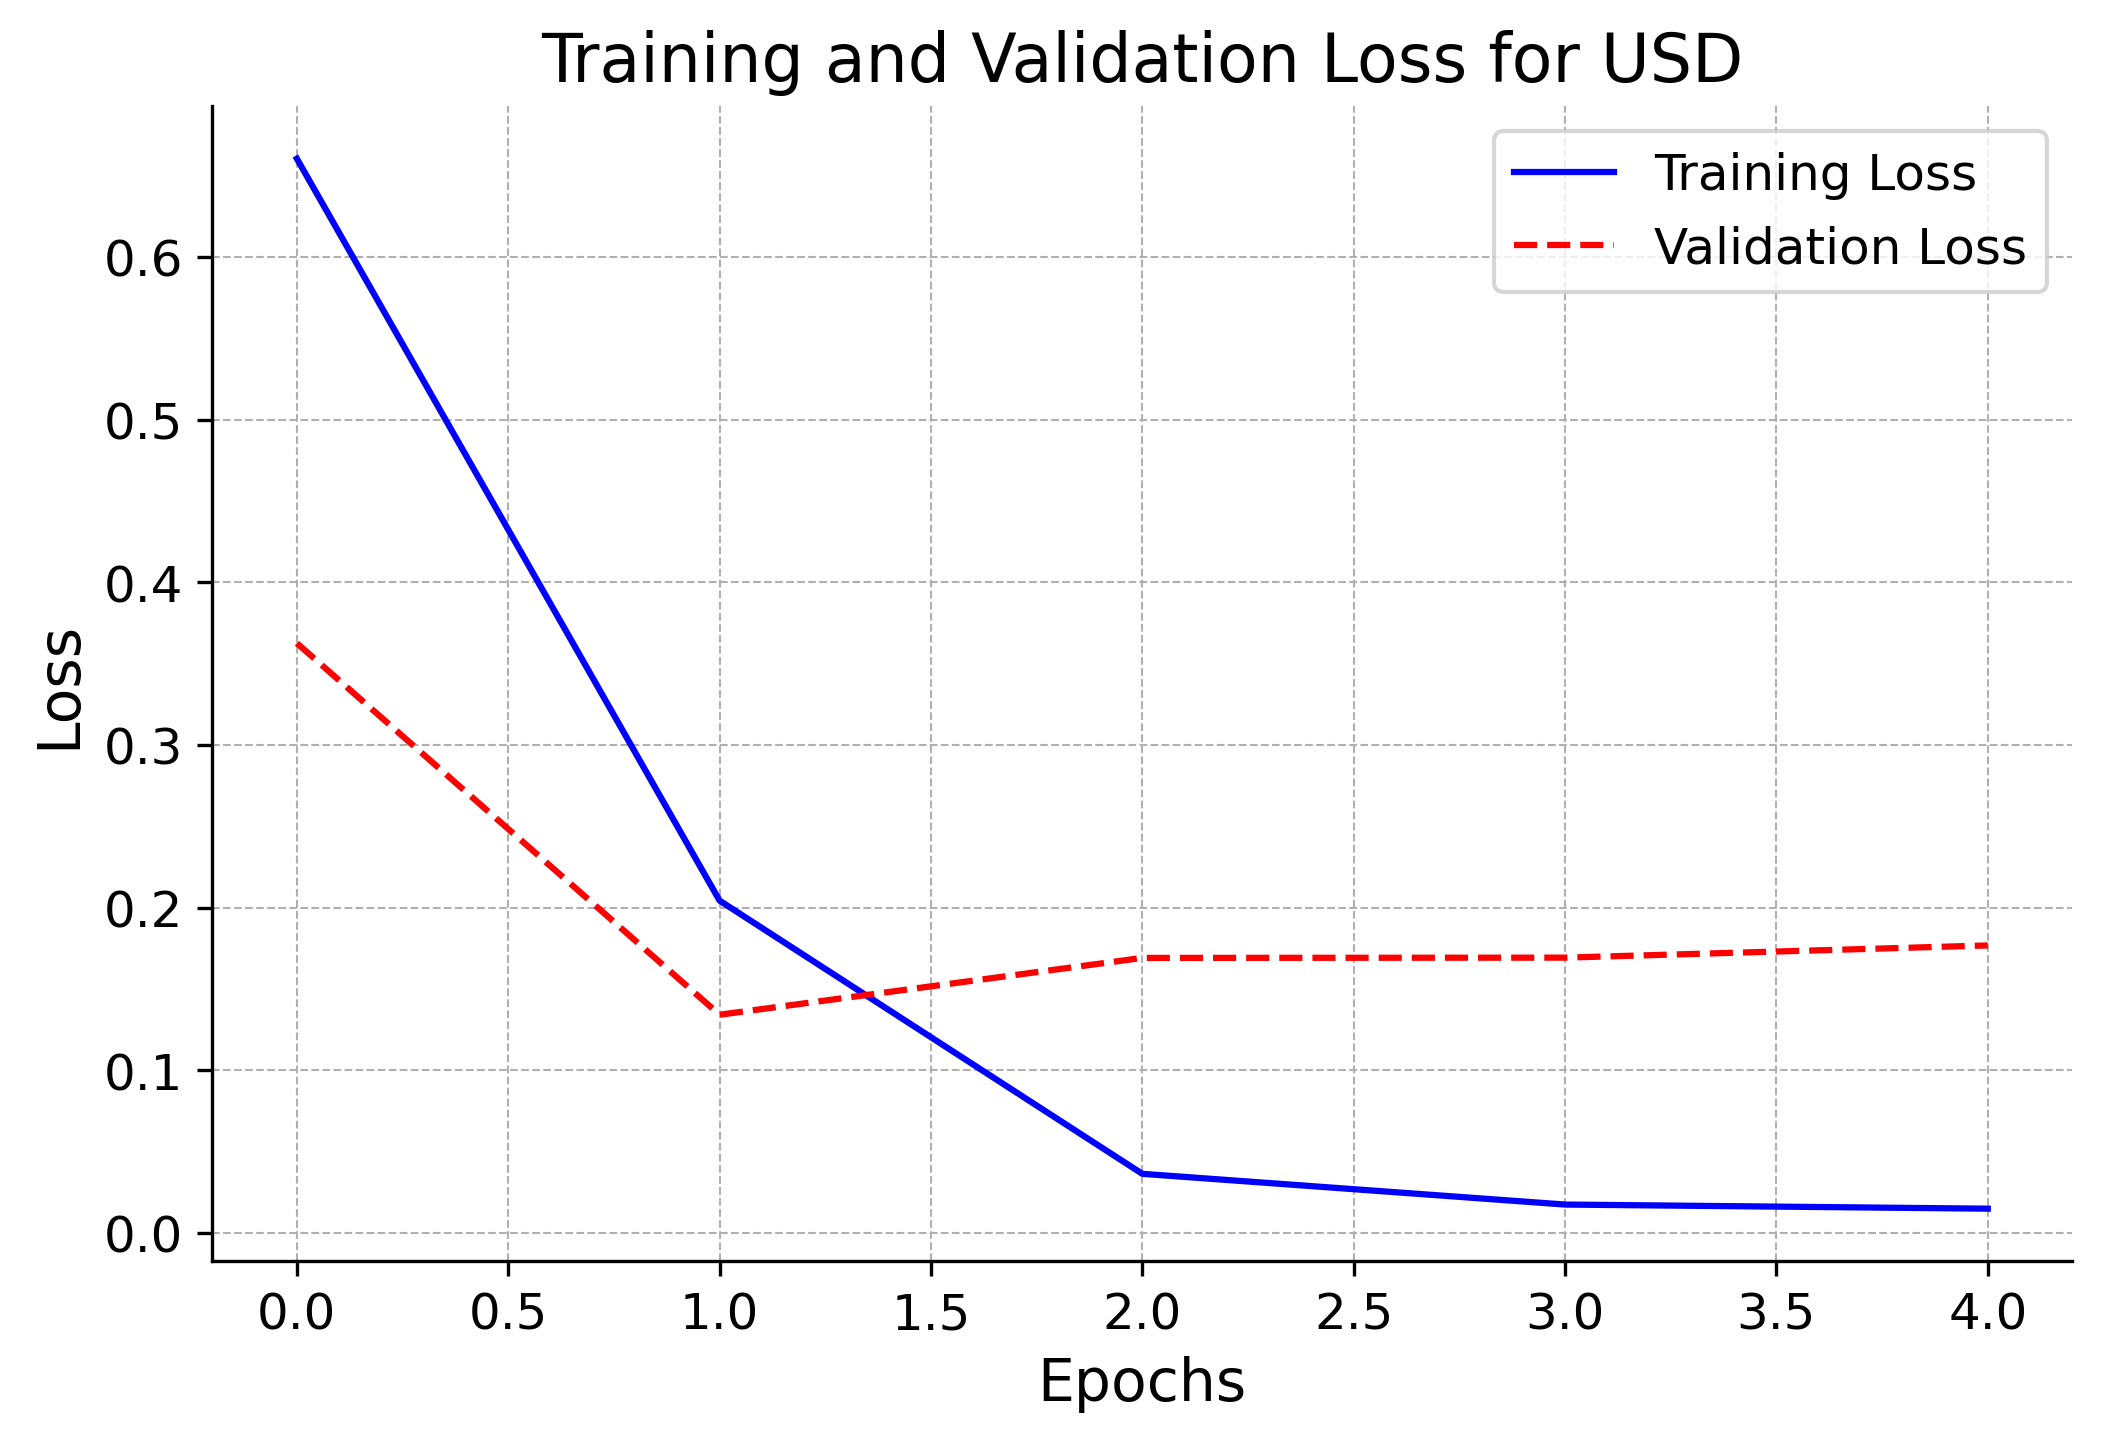
\includegraphics[width=\linewidth]{USD_loss_plot.png}}
\caption{Loss during ES-RNN training, for the USD, for a Weekly frequency.}
\label{fig:loss}
\end{figure}

The choice of choosing the L1 as the training loss function seems to have backfired. On a qualitative assessment, the system tended to have a positive bias (see Figure~\ref{fig:loss}). 

The above results emphasise the importance of having ample data when deploying hybrid algorithms, and suggests that traditional statistical methods can still hold their ground in such scenarios.

\section{Conclusions}

In this project we tried blending neural-network techniques with traditional statistical models for forex market forecasting. By using RNNs, CNNs, and Exponential Smoothing together, we hoped to improve predictions. However, our results showed that the V-AR outperformed both of the latter. The training loss function for the ES-RNN might not have been the best choice, as our system consistently leaned towards a positive bias, while the S-CNN did not seem able to handle non-stationary, and short data. In all cases, the old-school statistical methods worked better than the newer hybrid ones did. This tells us that having enough data is crucial, and sometimes, the simpler methods still work best.

\section*{Acknowledgments}

This report was typeset using \LaTeX, originally developed by Leslie Lamport and based on Donald Knuth's \TeX. A template that can be used to format documents with this look and feel has been released under the \href{https://www.ieee.org/publications/subscriptions/info/licensing.html}{\textsc{IEEE License}}, and can be found online at \url{https://www.overleaf.com/latex/templates/ieee-conference-template/grfzhhncsfqn}.

\begin{thebibliography}{00}
\bibitem{m4} S. Makridakis, E. Spiliotis, and V. Assimakopoulos, ``The M4 Competition: 100,000 time series and 61 forecasting methods,'' Int. J. Forecasting, vol. 36, no. 1, pp. 54--74, 2020. \url{https://doi.org/10.1016/j.ijforecast.2019.04.014}
\bibitem{smape} S. Makridakis, ``Accuracy measures: theoretical and practical concerns,'' Int. J. Forecasting, vol. 9, no. 4, pp. 527--529, 1993.
\url{https://doi.org/10.1016/0169-2070(93)90079-3}
\bibitem{mase} R. J. Hyndman and A. B. Koehler, ``Another look at measures of forecast accuracy,'' Int. J. Forecasting, vol. 22, no. 4, pp. 679--688, 2006.\url{https://doi.org/10.1016/j.ijforecast.2006.03.001}
\bibitem{es-rnn} S. Smyl, ``A hybrid method of exponential smoothing and recurrent neural networks for time series forecasting,'' Int. J. Forecasting, vol. 36, no. 1, pp. 75--85, 2020. \url{https://doi.org/10.1016/j.ijforecast.2019.03.017}
\bibitem{winters} P. R. Winters, ``Forecasting sales by exponentially weighted moving averages,'' Management science, vol. 6, no. 3, pp. 324--342, 1960. \url{https://doi.org/10.1287/mnsc.6.3.324}
\bibitem{e-cnn} A.P. Wibawa, A.B.P. Utama, H. Elmunsyah, et al., ``Time-series analysis with smoothed Convolutional Neural Network,'' J Big Data, vol. 9, pp. 44, 2022. \url{https://doi.org/10.1186/s40537-022-00599-y}
\bibitem{slawek} Slawek Smyl, Jai Ranganathan, Andrea Pasqua, ``M4 Forecasting Competition: Introducing a New Hybrid ES-RNN Model.''. Accessed 15 Sep 2023.\url{https://www.uber.com/en-GR/blog/m4-forecasting-competition/}. 
\bibitem{ayitey} M. Ayitey Junior, P. Appiahene, O. Appiah, et al., ``Forex market forecasting using machine learning: Systematic Literature Review and meta-analysis,'' J Big Data, vol. 10, pp. 9, 2023. \url{https://doi.org/10.1186/s40537-022-00676-2}
\bibitem{fletcher} TSB. Fletcher, ``Machine learning for financial market prediction,'' 2012, p. 207. \url{http://discovery.ucl.ac.uk/1338146/}. Accessed 15 Sep 2023.
\bibitem{islam} M.S. Islam, E. Hossain, A. Rahman, M.S. Hossain, and K. Andersson, ``A review on recent advancements in FOREX currency prediction,'' Algorithms, vol. 13, no. 8, pp. 1--23, 2020. \url{https://doi.org/10.3390/A13080186}.
\bibitem{ryll} L. Ryll and S. Seidens, ``Evaluating the performance of machine learning algorithms in financial market forecasting: a comprehensive survey,'' 2019. \url{http://arxiv.org/abs/1906.07786}.
\bibitem{panda} M.M. Panda, S.N. Panda, and P.K. Pattnaik, ``Exchange rate prediction using ANN and deep learning methodologies: a systematic review,'' in Indo-Taiwan 2nd International Conference on Computing, Analytics and Networks, Indo-Taiwan ICAN 2020—Proceedings, 2020, pp. 86--90. \url{https://doi.org/10.1109/Indo-TaiwanICAN48429.2020.9181351}.
\bibitem{brown} R. G. Brown, ``Exponential Smoothing for Predicting Demand,'' Cambridge, Massachusetts: Arthur D. Little Inc., p. 15, 1956.\url{https://www.industrydocuments.ucsf.edu/tobacco/docs/#id=jzlc0130}
\bibitem{ecb} European Central Bank, ``Euro foreign exchange reference rates,'' 2023. \url{https://www.ecb.europa.eu/stats/policy_and_exchange_rates/euro_reference_exchange_rates/html/index.en.html}. Accessed 15 Sep 2023.
\end{thebibliography}


\end{document}
